
\chapter{Relational Reinforcement Learning for Keepaway Soccer}


\section{Experiment}

\begin{figure}[h]
    \centering
    \begin{minipage}[t]{0.6\linewidth}
        \centering
        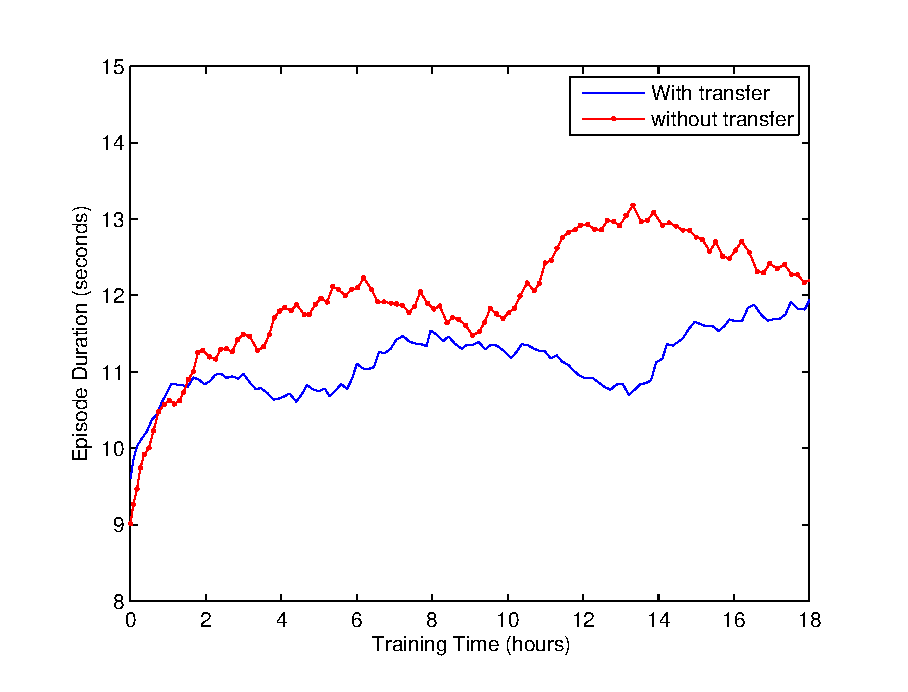
\includegraphics[width=\textwidth] {./figures/3vs2transfer.eps}
        \caption{The learning result of 3 vs 2 keepaway with/without prior training}
    \label{fig:3vs2transfer}
    \end{minipage}
\end{figure}

\begin{figure}[h]
    \centering
    \begin{minipage}[t]{0.6\linewidth}
        \centering
        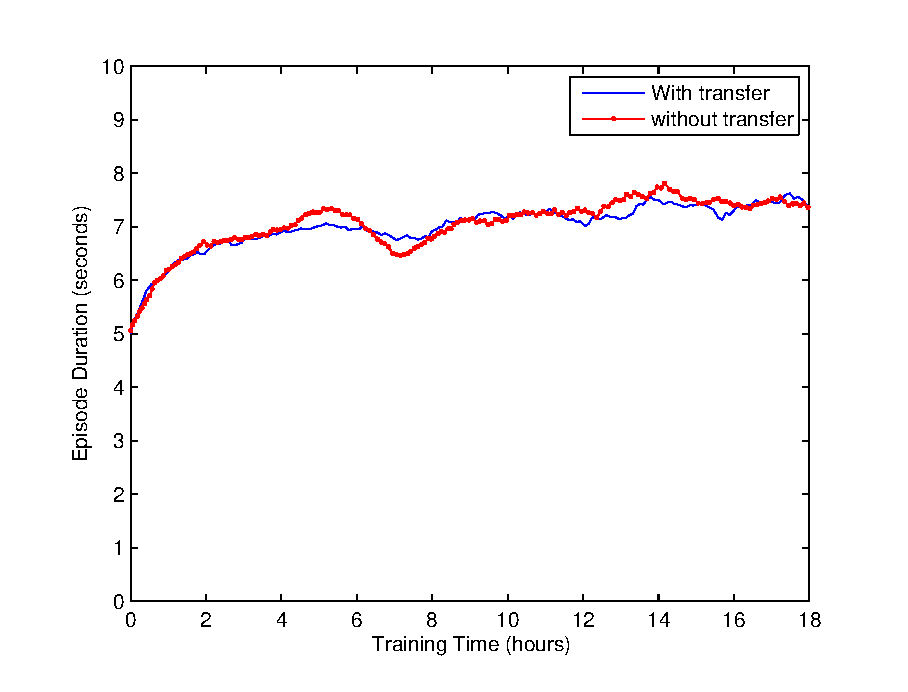
\includegraphics[width=\textwidth] {./figures/4vs3transfer.eps}
        \caption{The learning result of 4 vs 3 keepaway with/without prior training}
    \label{fig:4vs3transfer}
    \end{minipage}
\end{figure}

\begin{figure}[h]
    \centering
    \begin{minipage}[t]{0.6\linewidth}
        \centering
        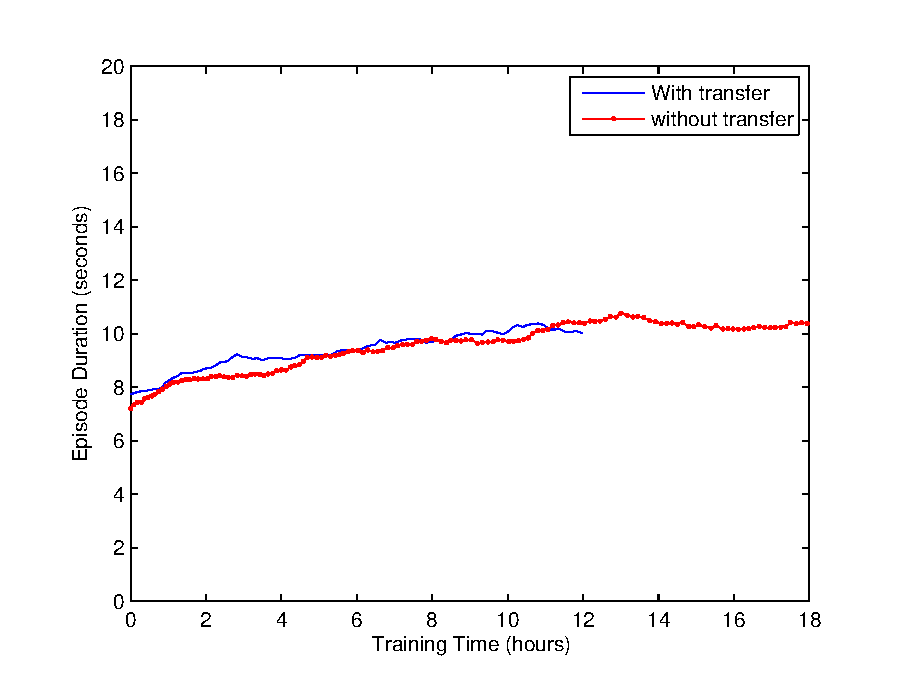
\includegraphics[width=\textwidth] {./figures/6vs5transfer.eps}
        \caption{The learning result of 6 vs 5 keepaway with/without prior training}
    \label{fig:6vs5transfer}
    \end{minipage}
\end{figure}
The experiment is performed in keepaway soccer simulator available at \\
(\url{http://www.cs.utexas.edu/~AustinVilla/sim/keepaway/}).
We first run the $SARSA(\lambda)$ to the 3 vs 2 keepaway soccer with all weights initialized to the highest possible reward (optimistic exploration). The exploration policy is 
the $\epsilon-greedy$ with $\epsilon$ set to 0.01. The temporal different coefficient $\alpha$ is set to 0.125 and the 
discount factor $\gamma$ is 0.95. The field size of the keepaway soccer is $20 \times 20$. 
The result is shown in Fig. \ref{fig:3vs2transfer} and \ref{fig:4vs3transfer}. 

To test our hypothesis, we then trained the agent in 1 vs 1 keepaway soccer for 200 episodes. 
In this simple scenario, the agent has no teammates, therefore the only action available to it is to hold the ball.
It helps the agent to learn the correct value for holding the ball all the times.
Clearly, the training of 1 vs 1 scenario is not enough for the agent to succeed since it does not know
when to pass the ball to its teammate. As a result, we use the knowledge of 1 vs 1 scenario as prior knowledge, 
and further trained it in 2 vs 1 keepaway for 1000 episodes.
With the knowledge about the 1 vs 1 and 2 vs 1 scenarios, the agent now can do better in 3 vs 2 and 4 vs 3 keepaway (Fig. \ref{fig:3vs2transfer} and \ref{fig:4vs3transfer})
than the untrained one.

\section{}
\[
   P(w, \mu, \Sigma| D) = P(D|\mu, \Sigma)P(\mu|w^Tu, I)P(w)\\
   P(w, \mu, \Sigma, h| D) = P(D|\mu, \Sigma)P(\mu|w^Tu, I)P(w|h)P(h)\\
   P(w, \mu, \Sigma, h| D) = P(D|\mu, \Sigma)P(\mu|h, I)\\
\]




























